In this introductory chapter, we motivate the study of social and economic dynamics from the complex systems' perspective. We begin by reviewing the scientific landscape in which this thesis is developed, and we introduce the challenges that the study of human behavior faces. This chapter aims to serve as a solid ground in which the concepts and tools employed in this thesis are positioned and understood, trying to make this thesis as self-consistent as possible. We introduce some basic concepts of complex networks, and we describe some tools that are used to model social and economic systems. Finally, we introduce the datasets that we use to study the temporal interactions in complex economic systems.

\section{\label{sec:scie_lands} Scientific Landscape and outline of the thesis}

This thesis addresses the study of human behavior and social systems from a \textit{complex systems} perspective, in which the emergence of collective phenomena, that arise from the interactions of many individuals, cannot be understood by studying the behavior of individual agents in isolation (the so-called \textit{reductionist} approach)~\cite{anderson1972more}. The study of collective phenomena has a long history in the natural sciences, specially in the branch of statistical physics~\cite{stanley1971phase}. This branch traditionally studies the emergence of collective phenomena in physical systems, such as the phase transitions in magnetic materials via spin models~\cite{onsager-1944}, the turbulence in fluids~\cite{frisch1995turbulence}, the synchronization in oscillatory systems~\cite{pikovsky2001universal}, or percolation~\cite{stauffer-1985}. However, in recent years, the study of complex systems has evolved into the study of emergent phenomena beyond physical systems, such as biological~\cite{brown2000scaling,aderem-2005,alon2019introduction}, ecological~\cite{may-2001}, economic~\cite{limburg2002complex}, and social systems~\cite{castellano2009statistical}. Even though this branch of physics is relatively young, in 2021, the Nobel Prize in Physics was awarded to Syukuro Manabe, Klaus Hasselmann, and Giorgio Parisi for their contributions to the study of complex systems~\cite{nobel-2021}, giving a recognition to this field in the scientific community~\cite{bianconi2023complex}.

From the migration of birds~\cite{roche-1997} to the spreading of fake news through social media~\cite{yamir-2004,vosoughi-2018}, there are many examples of collective phenomena beyond the realm of traditional physics at which the concepts and tools from complex systems and statistical physics can be applied~\cite{perc2013evolutionary}. The high share effects of renewable energy in power grids~\cite{maria-2023}, the spread of a disease in a population~\cite{anderson1991infectious}, the consensus in political elections~\cite{anderson-2000}, the emergence of social norms~\cite{ellickson-1999} are some examples of social or economic collective behavior in which the global phenomena cannot be understood by looking at a single individual. These collective human behavior has been studied from a variety of perspectives (sociology, psychology, economics, political sciences...), which often relies on qualitative methods, such as interviews, discourse analysis, or ethnographic studies~\cite{bryman-2010}. However, the complex systems' perspective aims to provide a quantitative framework to understand the collective behavior based on methodologies from statistical mechanics and network theory~\cite{newman-book,barabasi-2013}. This approach relies on the use of large amount of detailed data to extract significant correlations, validate theories and develop models. Reliable sources of human activity data have been a limitation to the study of social systems historically. It is in fact surprising how other branches of physics, where the typical scale of the phenomena is very large, as astrophysics, or very small, as particle physics, do not suffer from a lack of data, while the study of social systems, where the typical scale is human, has been historically limited by the lack of data.

Thankfully, the digital revolution has changed this picture, allowing the storage of large amounts of data generated by human activities, such as social media, mobile phones, or online platforms. Nowadays, every two year, more human socio-economic data is produced than during all the preceding years of human history together~\cite{karsai2019computational}. This data, often referred to as \textit{Big data}, has opened a new era for the study of social systems from a computational perspective, together with a paradigm shift in the way we understand human behavior~\cite{manyika-2011}. Nevertheless, this new era comes with an awareness, as the use of big data for the study of human behavior raises important ethical and privacy concerns, which need to be addressed in order to ensure the responsible use of data for the study of social systems~\cite{boyd-2012}. Moreover, from the technical point of view, this huge amount of data needs computational and mathematical resources to be analyzed and modeled. Satisfying this demand, the field of \textit{Computational Social Science} has emerged, with the aim to develop new methods to study human behavior from real data significant correlations~\cite{Lazer2009CompSocSci}. This branch of the complex systems science was born as a combination of methodologies borrowed from social sciences, such as sociology, psychology, or economics, with computational methods from hard sciences (physics, mathematics, computer science)~\cite{watts-2007}, such as network theory, statistical mechanics, machine learning, data mining, etc. This interdisciplinary approach has allowed developing new methods for forecasting social phenomena and understanding the basic mechanism behind human interactions. 

One can differentiate two main approaches to build a modeling framework from the data source. The first focuses on the prediction and forecasting of a certain social phenomenon, such as the spread of a disease or the price of a stock. In this approach, the data is seen as a necessary input to our methodology to make quantitative predictions~\cite{Lazer2009CompSocSci}. However, in this approach, the mechanisms behind the phenomena are often hidden in the data, and the model is seen as a black box that provides accurate predictions~\cite{rudin-2019}. In this context, the use of machine learning~\cite{murphy-2012} and deep learning~\cite{goodfellow-2016} models are  very popular, as they are able to capture complex patterns in the data and reproduce it with high levels of accuracy. The second approach is to focus on the understanding of the mechanisms behind the phenomena. In the later approach, the data is seen as a problem to be understood, an observation from which we can extract qualitative behaviors and patterns~\cite{axelrod2006agent}. In this context, the aim is to develop very simple models that are able to reproduce the main features of the data, and to extract the basic mechanisms behind the phenomena.

Following the second approach, network science has a critical role in the study of socio-economic systems, as it provides a natural framework to study the interactions between individuals. A network, or graph, is a mathematical representation of a set of nodes connected by links or edges, which allows to study the structure of the interactions between the different elements. The study of networks has a long history in the natural sciences, from the neurons network in the brain~\cite{sporns-2004} to food webs in an ecosystem~\cite{ings-2008, elith-2009, bastolla-2009}. However, in recent years, new data sources lead to the discovery that complex properties and heterogeneity, present in most social systems, need for a topological description in terms of a complex network~\cite{newman-book, dorogovtsev2002evolution, boccaletti2006complex}. Social networks, such as a social media~\cite{dunbar-2015}, the collaboration network of scientists~\cite{newman-coll-2001,radicchi-2008}, or international conflicts~\cite{hafnerburton-2009, diaz2023network}, are found to exhibit non-trivial topological properties and often are referred as \textit{complex networks}, which will be explained later on this chapter. In particular, the study of information spreading as a dynamical system is an example of a system in which network theory has allowed to understand how information spreads and how consensus emerges (and if it does).

Spreading of information has been a topic of interest for many social scientists. Early theoretical frameworks, influenced by psychological and sociological theories, show how individuals in a crowd lose their sense of self and are more susceptible to the ideas and emotions of the crowd~\cite{le2023crowd}. Social imitation of behaviors and ideas was proposed as a mechanism for social change, facilitated by close contact and communication among individuals~\cite{kanter-1971}. Similarly, peer pressure was also proposed another possible mechanism, where individuals are influenced by their peers to adopt certain behaviors or ideas~\cite{granovetter-1978, brown-1986}. However, until now, these theoretical dissertations were not supported by quantitative results with real data analysis (besides controlled experiments). The spread of innovations~\cite{rogers2014}, the diffusion of information~\cite{valente-1996}, or the spread of diseases~\cite{anderson1991infectious} are some examples of social phenomena where the traditional theoretical frameworks can now be tested or modified to explain correlations observed from data sources.

Beyond the network structure and the contagion dynamics, there is a third ingredient that is critical for the study of human dynamics: the temporal patterns. Human interactions exhibit complex activity patterns that are difficult to understand and to model, since there are a lot of mechanisms that drive the human behavior. For example, the circadian rhythms~\cite{roenneberg-2013}, bursty interactions~\cite{Barabasi2005Bursts}, cascades~\cite{watts-2002}, periodic commuting behaviors~\cite{gonzalez2008understanding}, recurring patterns in online behavior~\cite{Lazer2009CompSocSci}, etc., are effects embedded to the socio-economic environment and the social network structure, so they cannot be ignored. In fact, through this thesis, we will show how the temporal patterns of human interactions affect processes such as information spreading ~\cite{Holme2012Temporal}, changing the nature of the dynamic process dramatically~\cite{karsai-2011}.

In this thesis, we use the complex systems approach to try to understand the consequences of the irregular human activity patterns (temporal interactions) in socio-economic models. In the first part of the thesis, we incorporate memory effects associated with aging to models where social change is driven by peer-pressure (\textit{threshold models}). Modelling in this part of the thesis is seen as a tool to understand the basic mechanisms behind the phenomena and to extract the main features of the data, not with the aim to make accurate predictions. Under this perspective, we will apply tools borrowed from computational social science, network theory and statistical mechanics to study some problems under this umbrella: the emergence of segregation, the spreading of information and the consensus problem. In the second part, data from a real economic system takes a relevant role. We use a dataset of listings from a real estate platform from which, via network theory, we extract the relevant information about the temporal interactions in the system, highlighting the memory effects. In particular, we develop a methodology to address the spatial segmentation and the decision-making mechanisms present in the housing market.

\subsection{\label{sec:Thesis outline} Thesis outline}

This thesis is divided in 3 main parts:

\begin{itemize}
    \item In the \textbf{Introductory part}, we explain the basic concepts necessary to understand the findings in this thesis. Chapter 1 introduces the field in which this thesis is developed. Network theory and agent-based modeling are also introduced in this chapter. Chapter 2 describes and reviews the so-called threshold models for this thesis, and introduce the notion of burstiness and aging in the socio-economic context. 

    \item In \textbf{Part I}, we investigate the aging implications in threshold models. We will see that aging has been proposed as a possible explanation to the heterogeneous human activity patterns. We explore how aging modifies the threshold model dynamics in 3 different threshold models designed for 3 different social systems. In Chapter 3, we study the aging implications in a popular segregation model. In Chapter 4, we introduce a new mathematical framework to include aging in binary state dynamics, which is applied in Chapters 5, to see the aging effects in a complex contagion model, and in Chapter 6, to explore aging in a consensus model. Chapter 6 is divided in two main ``subchapters'': The first one dedicated to understand the phase diagram of this consensus model and the second one to explore the aging implications in both the statics and dynamics of the model.
    
    \item In \textbf{Part II}, we study the temporal interactions in a real economic system. We will see an example of irregular temporal patterns in the housing market via the listings from an online platform.  From this data, Chapter 7 analyzes the statics of the system, exploring how the real estate agencies specialization segments the housing market. Following this approach, we develop a methodology to assess this segmentation, which is found to be robust in the different markets. In Chapter 8, we will analyze the dynamics of the listings, focusing on which mechanisms drive the decision-making process of house sellers when they choose a real estate agency to sell their property. 
    
    \item Finally, in the \textbf{Part III}, we summarize the main findings of this thesis and discuss the implications of the results in the field (Chapter 9). In Chapter 10, we discuss the limitations of the study and propose future possible research along the lines of this thesis.
\end{itemize}

\section{\label{sec:Challenges of Computational Social Science} Challenges of Computational Social Science}

Since the research in Computational Social Science is relatively new, the methodology is not yet well established, but follows the traditional approach from natural sciences, like physics, but with new relevant techniques adapted to the specific problem to address. In this section, we introduce some challenges the study of human behavior faces, and how these challenges are addressed in the context of our research.

Regarding the \textbf{data availability}, digital behavioral data provides a detailed look at human activities in their usual environments, capturing information about where, when, and how people behave~\cite{Eagle2006RealityMining}. This type of data is great because it avoids the common biases seen in older research methods, such as surveys, and gives us a clearer picture across a large number of people~\cite{Lazer2009CompSocSci,chen-2014}. Instead of relying on limited lab studies or broad census data, the data is now collected from real-world interactions, stored from digital devices and platforms that people use in their daily lives~\cite{Eckmann2004Entropy,blondel-2015,artime-2017}. However, this data is similar to a picture of a black hole, neither you can observe it in a controlled environment nor it is possible to analyze the response to a stimuli~\cite{lazer-2014}. Also, not everyone is equally represented in digital data, especially in underdeveloped countries, where the use of recent technology is less popularized~\cite{zook-2017}. Ethically, there are also big concerns about collecting and using personal data without people knowing it~\cite{boyd-2012, de-montjoye-2013}, which has pushed for stricter laws to protect privacy and ensure people have control over their own data.

Regarding  \textbf{data analysis}, few decades ago several statistical methodologies were designed to manage small data sets in social and economic research, giving rise to meaningful models and techniques~\cite{stevens-2012, gelman-2006}. These traditional techniques have evolved to accommodate the large data volumes seen in modern statistical analysis~\cite{hastie-2013}, where the challenge is no longer sample size but the data heterogeneity. Using tools such as data mining, data curation and statistical tests, we can convert large noisy data sets into intelligible knowledge from which extract significant patterns~\cite{witten-2005}. Furthermore, network analysis is helpful to analyze several datasets from a different perspective, highlighting the crossed interactions between the different elements~\cite{newman-book, clauset-2008}. The use of null models~\cite{perry2012null,gauvin-2022} is an example of a common practice in network analysis, in which the interactions are rewired (reshuffled), breaking the correlations, such that we can discriminate if the macroscopic properties of the network are meaningful or not.

Regarding to \textbf{understanding and modelling human behavior}, there are 3 main approaches one can follow: Statistical Models are used to identify correlations and make individualized predictions. For example, machine learning~\cite{murphy-2012}, Bayesian inference~\cite{gelman1995bayesian}, deep learning~\cite{goodfellow-2016}, etc. Mechanistic Models, inspired by physics, simulate emergent behaviors from simpler entity interactions, offering robust scenario testing but often simplifying individual differences~\cite{axelrod2006agent}. Agent-based modeling (ABM) emerged as a particularly influential mechanistic approach, enabling scientists to create and study systems of interacting agents (individuals or collective entities) and observe emergent behaviors from simple rules of interaction~\cite{epstein1999agent}.On the other hand, Data-driven Models blend real-world data with synthetic frameworks to focus on specific mechanisms, allowing for realistic simulations and in-depth analysis of the dynamics. The availability to address problems from these 3 perspectives is crucial in an interdisciplinary field as computational social science, and enhances understanding by forming, testing, and refining hypotheses~\cite{watts2004new}.

Finally, the scope of \textbf{applications} in Computational Social Science is very broad, including managing crowd dynamics, improving cooperative behaviors, optimizing traffic and public transport systems, facilitating product and service adoption, and forecasting global pandemics. This multifaceted field is becoming increasingly relevant in modern techno-social societies~\cite{vespignani2009predicting}, enhancing the quantitative nature of social sciences and leading the shift towards a digital, data-driven paradigm across science, technology, and various applied domains. One example of these applications, related to contagion dynamics, are the fake news observatories~\cite{Polis-observatory, EDMO-observatory, committed-observatory-2023}, which are platforms that monitor the spread of fake news in social media, and provide tools to detect and give feedback to the users.

\subsection{Thesis positioning in Computational Social Science\label{subsec:Thesis positioning in Computational Social Science}}

Through this thesis, the main challenge faced is the understanding and modeling of human dynamics. In the first part of the thesis, the data is used primarily as inspiration to develop reasonable models that explain the emergent properties of the data. We use tools borrowed from network theory and statistical mechanics to study the impact of aging on social processes driven by peer pressure, focusing on the emergence of segregation, the spread of information, and the consensus problem. The main challenge addressed in this part of the thesis is modeling the non-Markovian nature of human dynamics. The aging mechanism introduces a memory effect in the system, preventing us from using traditional tools to describe Markovian dynamics. Therefore, throughout the thesis, we extend mathematical frameworks to a formulation that allows us to describe the dynamics of non-Markovian binary-state models in complex networks.

In the second part of the thesis, we use a real dataset from an economic system. The main challenge addressed in this part is data curation and the analysis of temporal patterns and correlations. The dataset comprises listings from a real estate platform, containing information about interactions between sellers and real estate agencies during a period of time. We use network theory to extract relevant information from the data and develop a methodology to address spatial segmentation and decision-making mechanisms in the housing market. The main challenge in this part of the thesis is the development of new methodologies to extract relevant information from the data and the creation of new algorithms for clustering and studying the system's dynamics. However, there is also modelling involved, since this part is related with the first part of the thesis precisely because one can understand the temporal irregularities in the housing market as an aging/resistance mechanism.

\section{\label{sec:Terminology and general concepts} Terminology and general concepts}

Here, we briefly introduce general definitions and concepts, which will be used through the thesis. We introduce basic concepts of complex networks, and modeling techniques used in the study of social and economic systems.
\subsection{\label{subsec:Complex networks} Complex networks}
A network is a mathematical representation of a set of nodes connected by links. This simple definition allows to map the architecture of many complex systems by identifying the interactions between the different elements. This topology allows us to quantify how close or far two nodes are, how central a node is, how dense a system is, etc. As I understood it through these years,  what makes a network complex in my opinion is having a short path length, such that average distance between two nodes is relatively small, high levels of clustering, result from a triadic closure effect, and a scale free degree distribution, such that several nodes with low degree coexist with few nodes with a very high degree. These properties are often found in many social, biological and economic complex systems, such as social media, ecological networks, or financial systems.

To create synthetic networks with the same properties as real complex networks, we use stochastic models that, from few nodes, describe how we need to grow the network to reach our goal~\cite{posfai2016network}. Historically, the first attempt was the Erd\H{o}s-Renyi (ER) model~\cite{erdos1960evolution}, which grows the network by simply adding links between nodes with a certain probability $p$. This model is useful to study the emergence of the giant component in a network, which is the largest connected component in the network (see an ER network in Fig. \ref{fig:netwotk_types}a). However, as a result of this process of adding links according to $p$, the degree distribution is a binomial distribution, and the clustering, which decays with the network size $N$ as $p/N$, is too low to reproduce a real complex network. Another popular example is the Watts-Strogatz model~\cite{watts1998collective}, which starts from a regular network, typically a ring lattice, and rewires the links with a certain probability $r$. This model is useful to study the emergence of small-world networks, which have a short path length and a high clustering. However, rewiring does not change the degree distribution, so it is still binomial, which is a limitation to reproduce the fat tail distribution found in real complex networks~\cite{newman2003structure}. The Barab\'asi-Albert model~\cite{barabasi1999emergence} grows the network by adding nodes that attach to the present nodes with a probability proportional to the degree of the nodes. This process is called \textit{preferential attachment}, and it is known to be useful to reproduce the fat tail distributions~\cite{merton1968matthew} or, in other words, the emergence of hubs (nodes with a very high degree) in a network (see Fig. \ref{fig:netwotk_types}b). If instead of adding nodes according to a certain rule, we want to directly impose a certain observed degree distribution, we can use the configuration model~\cite{newman-book}, which is a generalization of the Erd\H{o}s-R\'enyi model in which we start from a set of nodes disconnected, each one with a certain number of stubs, and then we connect the stubs with a certain probability. It can be shown that the clustering in networks generated using the configuration model for any degree distribution is proportional to $1/N$, where $N$ is the number of nodes in the network. This means that for large networks, the clustering is very small, a feature that we will see may be useful to describe agent based models in networks.

Until now, we considered only simple networks, in which the links are binary (there is link or there is not). However, we can consider that links are weighted, which means that each link has a certain number (or another quality) associated to it~\cite{barrat2004architecture} (see Fig. \ref{fig:netwotk_types}c). This representation is useful to describe the strength of the interactions between nodes. For example, the railway network is a simple network that connects stations via the railway lines, but the weight of each line could be number of trains or the number of passengers that travel through it~\cite{latora-2002}. This representation is very useful when we have a system very densely connected, but there are some links that have a higher importance or are more saturated than others, depending on the context. Also, this representation allows us to map any correlation matrix as a weighted network, which might be useful to identify the more correlated and anticorrelated elements in a system~\cite{onnela-2003,tumminello-2005}.

\begin{figure}
    \centering
    % Set the caption fony to cmss using tgbonum package
    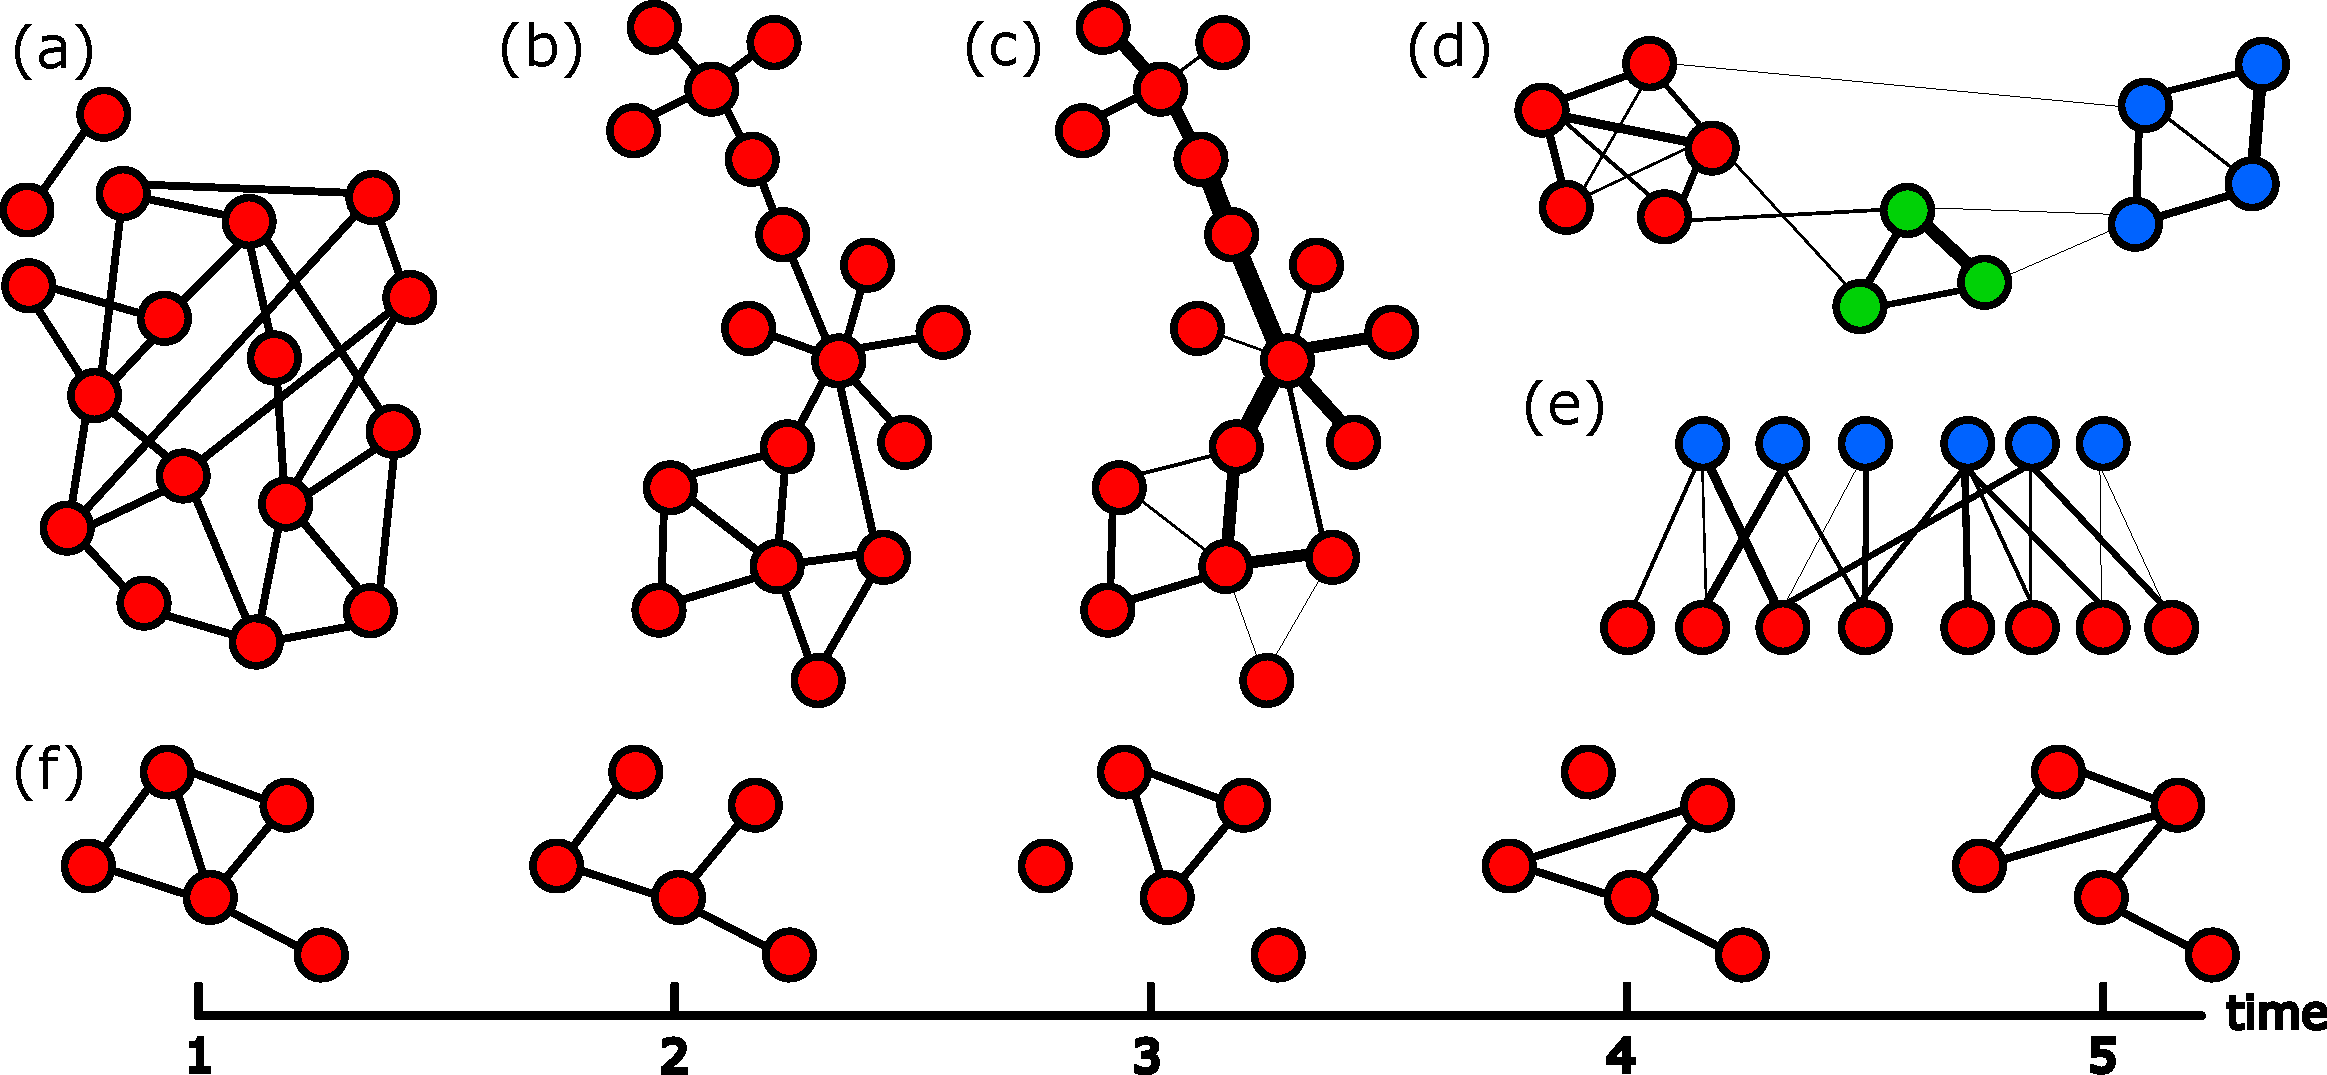
\includegraphics[width=\textwidth]{Figs/Introduction/network_plot.pdf}
    \caption[Different network types]{Representation of some different types of networks: \textbf{(a)} Simple Erd\H{o}s-R\'enyi network, \textbf{(b)} Simple Barab\'asi-Albert network, \textbf{(c)} Weighted Barab\'asi-Albert network, \textbf{(d)} Weighted network with community structure, \textbf{(e)} Weighted bipartite network and \textbf{(f)} Simple temporal network evolving during 5 time steps. The nodes are represented by colored circles, and the links are represented by lines, where the width of the line represents the weight of the link. In (d) the color of the nodes represents the community to which they belong and in (e) the type of the nodes to which they belong.}
    \label{fig:netwotk_types}
\end{figure}


In fact, a common trait that is found in complex systems is the presence of communities, which are groups of nodes that show a favoring bias to connect with nodes of the same group~\cite{girvan-2002} (see Fig. \ref{fig:netwotk_types}d). For example, communities can represent groups of friends, families, or work colleagues, which are more likely to share information and to interact between them~\cite{newman2003structure}. To identify communities in a network, we can use community detection algorithms, which are computational tools that group nodes in the network in a way that maximize the community structure, such as maximizing the number of links inside the groups and minimizes the number of links between the groups~\cite{lancichinetti-2008,fortunato2010community}. One popular example is the Louvain algorithm~\cite{blondel-2008}, which is a greedy algorithm that optimizes the modularity function, which is a measure of the quality of the partition of the network. Another popular example is the Infomap algorithm~\cite{rosvall-2008}, which is a flow-based algorithm that optimizes a map equation, which is a measure of the quality of the partition of the network. Another recent example more sophisticated is the OSLOM algorithm~\cite{OSLOM}, which is a stochastic algorithm that optimizes the likelihood of the partition of the network and is able to identify overlapping communities. These algorithms are useful to identify the structure of the network, and to understand the dynamics of the system.

On the other hand, there are networks in which by definition there are two natural types of nodes, and there are just links between the two nodes of different types (not between nodes of the same type). These networks are called bipartite networks~\cite{newman2003structure}, and they are useful to represent systems in which there are two types of elements, and there are only interactions between them~\cite{latapy-2008} (see example in Fig. \ref{fig:netwotk_types}e). For example, online platforms to see movies and TV shows, such as Netflix~\cite{netflix} and HBO~\cite{HBO}, can be considered as bipartite network in which there are users and movies, and there are links between users and movies if the user has watched the movie. This representation is useful to study the recommendation systems based on the user preference~\cite{ricci-2011}. Moreover, bipartite networks allow us to project into a weighted network of nodes of the same type, where the weight of the link is typically computed and normalized by the number of common neighbors (of the other type) between the two nodes~\cite{newman-2001-collaboration}. In the case of the movie recommendation system, we can project the bipartite network into a weighted network of users, where the weight of the link between two users is the number of movies that they have watched in common. The projection is useful to study the social interactions between users, and to identify communities in the network.

Finally, there are networks in which the interactions between nodes are not static, but they evolve in time (temporal networks)~\cite{Holme2012Temporal} (see evolution of a simple network in Fig. \ref{fig:netwotk_types}f). These networks are useful to represent systems in which the interactions between nodes change in time~\cite{Perra2012ActivityDriven}. For example, the phone calls in a group of friends is a temporal network, in which the links are the phone calls that take place at a certain time window. This representation is useful to study the dynamics of the system, and to understand the network activity~\cite{karsai-2011} or if there are periodic patterns~\cite{Jo2012Circadian}.

Through this thesis, the types of networks described above will be used to model the interactions between the agents in the system, and to understand the dynamics of the system. In the first part of this thesis, we just use artificial simple networks created via the models described above. However, at the second part, we use bipartite network (weighted and unweighted), projected networks, community detection algorithms, and temporal networks to study the dynamics of a real economic system. 

Besides these networks representations, there are plenty of other types of networks very popular to describe social and economic complex systems. One important example are multiplex networks~\cite{gomez-2013,kivela2014multilayer,de2013mathematical}, which are networks in which there are several layers of interactions between the nodes. This representation is useful to study the interplay between the different layers of interactions. Another example is the network of networks~\cite{gao2011robustness, d2014networks}, which are networks in which there are several networks that are interconnected between them. There are hypergraphs (or higher-order networks)~\cite{battiston-2021}, which are networks in which the links are not between two nodes, but between a set of nodes, and signed networks~\cite{leskovec2010signed}, which are networks in which the links can be positive or negative. 


\subsection{\label{subsec:Agent-based models} Agent-based models}

Agent-based models are a class of computational models for simulating the actions and interactions of autonomous agents such that we can assess their effects on the system as a whole~\cite{duffy-1998, bonabeau-2002}. In the context of our thesis, agent based models are used to understand the collective behavior of the agents and the emergent properties of the system from a simple set of rules. Agents can be individuals, groups, or organizations, and if the network topology is necessary, the agents are placed in the nodes of a network~\cite{macal-2010, railsback-2011}. The agents are characterized by its state, which may be a set of  discrete or continuous variables, and its behavior or update rules. The rules, deterministic or stochastic, are the recipe that the agents need to follow to interact with its environment. For example, for the Voter model, an agent has a state that represents one of the two opinions and the update rules are just to imitate the state of a neighbor~\cite{castellano2009statistical}. Despite these simple rules, the Voter model shows a very rich phenomenology which nowadays is mainly studied via agent-based simulations.

An important ingredient when we perform agent-based simulations is the order in which nodes are updated. The order can be synchronous, in which all nodes are updated at the same time, or asynchronous, in which nodes are updated one by one~\cite{macal-2010, railsback-2011}. Nevertheless, the synchronous update may lead to problematic schemes, in which the system may get stuck in a periodic or chaotic solution. Performing simulations in asynchronous order, the order can also be random, in which nodes are updated one by one in a random order, or sequential, in which nodes are updated in a certain order. A common order is to just follow a random asynchronous update (RAU), which avoids biases and allows to explore the space of solutions in a more efficient way. Nevertheless, the sequential asynchronous update (SAU) is useful to reduce the computational cost, because going through the system sequentially may lead faster to the stationary state.

Usually, in agent based-models, these simulation steps are repeated until a stationary state is reached (if exists). To do so, one can perform Monte Carlo simulations~\cite{metropolis-1949,cronin2006monte}, which are a class of computational algorithms that rely on repeated random sampling for many time steps to reach the stationary state. In these simulations, a time step (Monte Carlo step) is defined as the time in which, on average, each node is updated once~\cite{newman-1999, landau-2014}. These are useful to explore the space of solutions, and to understand the dynamics of the system. A different approach is to use the Gillespie algorithm~\cite{gillespie-1977}, which is a stochastic simulation algorithm that generates a trajectory of the system by sampling the time of the next event and the event that will take place. This algorithm is useful because, since the time is not fixed, we avoid time steps in which nothing happens, and we can explore the dynamics of the system in a more efficient way~\cite{gibson-2000}.

Finally, the output of these simulations is a set of relevant statistics that describe the system's trajectory or the stationary state. These statistics can be the average opinion of the agents, the number of clusters, the number of links between clusters, the average interface density, etc. An ensemble of simulations is often performed to explore the space of possible trajectories and solutions, and to understand the robustness of the results. This ensemble can be performed by simply repeating the stochastic simulation, or by changing a trait of the system, such as the initial conditions of the system, or the realization of the network. This procedure is repeated for the relevant parameters of the model to explore the phase diagram, a methodology borrowed from statistical physics that refers to the parameter space in which, for each set of parameter values, we can identify the stationary solution~\cite{goldenfeld-1992}.

\section{\label{sec:Datasets} Application to a real case scenario}

\begin{figure}[ht]
    \centering
    \includegraphics[width=0.80\textwidth]{Figs/Introduction/adds_size_map.pdf}
    \caption[Listings distribution in space]{Distribution of the listings in the dataset in the Spanish provinces of Balearic Islands \textbf{(a)}, Barcelona \textbf{(b)}, and Madrid \textbf{(c)}. The space is divided into $1 \times 1$ km$^2$ cells. The color of each cell is the natural logarithm of the number of listings in the cell. The maps show that the listings are concentrated in the city centers. }
    \label{fig:maps_adds}
\end{figure}

\subsection{\label{subsec:Idealista dataset} Idealista dataset}

A central part of research in computational social sciences is the use of data to validate theories and develop models to understand the dynamics. In the second part of the thesis, we used mainly one dataset to study the temporal interactions in a complex economic system. This is a dataset of listings published on the online platform \texttt{Idealista.com}~\cite{idealista}, which is a Spanish real estate platform that connects buyers and sellers of real estate properties. The dataset covers a 2-year time period, from January 2017 to December 2018, and it comprises a comprehensive collection of online listings georeferenced with their (lat, long) coordinates in the Spanish provinces of Balearic Islands, Barcelona, and Madrid. These listings were posted by more than $50,000$ real estate agencies, each identified with its unique ID. For each listing, we have information about the price of the property, the type of property (flat, house, etc.), the number of rooms, the surface of the property, the real estate agency that posted the listing, and the dates at which the listing was posted and removed. This dataset comprises over one million listings for sales, and over $800,000$ for rentals. We focus on houses and apartments, and do not consider farms or rural parcels and remove listing with missing information or with an irregular price. The dataset is a snapshot of the real estate market in the 3 Spanish provinces, and it allows us to study the dynamics of the market, the interactions between the real estate agencies, and the emergence of spatial correlations. See Fig. \ref{fig:maps_adds} to see the irregular distribution of the listings in the space for the Spanish provinces of Balearic Islands, Barcelona, and Madrid.

The exploration of this dataset is an interesting case study because it provides a detailed, comprehensive view of the real estate market in key Spanish provinces, which a large metropolis in each province, over a substantial period. The high accuracy georeferenced nature of the data enables sophisticated spatial analyzes, uncovering regional patterns and disparities. This dataset not only aids in validating economic theories and developing predictive models but also offers valuable insights for policymaking, business strategy formulation, and academic research in computational social sciences. On the other hand, it has several limitations. First, the dataset only covers listings from a single platform, potentially missing data from other real estate websites or offline sources, leading to a biased view of the market~\cite{gonzalez2014assessing}. Additionally, the dataset spans just two years, which may not capture long-term trends or the impact of economic cycles. It is worth also to mention that the dataset reflects only the listings, providing a picture of the market's offer side but not the actual transactions, limiting insights into the full market dynamics. These limitations must be considered when interpreting the results and making broader generalizations.

\subsection{\label{subsec:SeLoger dataset} SeLoger dataset}

Moreover, for test properties of the real estate market spatial segmentation, we used a French dataset of listings posted on the online platform \texttt{SeLoger.com}~\cite{SeLoger}. This dataset covers a 6-month time period, from July to December 2019, including over 2 million sale listings across 3 French urban areas: Paris, Marseilles, and Toulouse. These listings are geolocalized by ZIP codes (``\textit{code postal}''), municipalities (``\textit{communes}''), and census tracts (``\textit{IRIS}''), the finest and basic scale for sub-municipal information in France (the lat-long coordinates of the listings are not available). For each listing, we have information about the price of the property, the type of property (flat, house, etc.), and the real estate agency that posted the listing. We focus on houses and apartments, and do not consider farms or rural parcels and remove listing with missing information or with an irregular price, as we did for the Spanish dataset.